\section{Locomotion Mode}
We construct a Locomotion Mode as a collection of optimizable primitives, where each $\prim^{d,p}_v$ containts $d$ optimizable parameters, takes $p$ values as input, and outputs a single return value. We implemented 3 primitive types as constant, 1DBlendSpaces and 2DBlendSpaces as illustrated in fig ???. These primitives have the advantage that optimization is readily possible, while the exposed parameters and their effetcs on the blend spaces are familiar to animators.
It is possible to build many different types of Locomotion Modes from these simple primitives. For plane locomotion we use:

Avantage that the primitiv are differntiable !


\section{Movement Model}

A movement model describes how an entity moves through space given control input. It consists of internal parameters such as velocities and accelerations. Control input could be a direction of movement supplied by a human using a gamepad, or longer paths supplied by a game engine AI system.

We have not seen any formal description of the movement model. Ususally some ad hoc newtonian physics concepts are combined with springs and animation curves to control the system.

In the following we limit the description to locomotion in the plane. 

We parameterize the movement model as $\mathcal{M}=L,T$ where $L=l_0 \ldots l_n$ is a set of locomotion modes and $\mathcal{I}=i_0 \ldots i_m$ is a set of interpolators that describes the transition between locomotion modes. A movement model defines the behaviour of an actor $\mathcal{A}=\boldsymbol{\omega},p,\dot{p},r,\dot{r}$ where $p$ and $r$ describe position, orientation and their derivatives.  $\boldsymbol{\omega}=\omega_0 \ldots \omega_n$ contains contribution weights for $l \in \mathcal{L}$. Notice $||\vec{\boldsymbol{\omega}}||^2=1$ and usually only a couple of modes will be active as in a transition between walking and running where $\boldsymbol{\omega}=\omega_{walk}:0.8, \omega_{run}:{0.2}, \omega_{other}:0$

An actor is moved with a control signal $\mathcal{C}=l_c, u, \Delta{t}_c, p_c,r_c$ containing locomotion mode, interpolation weight, timestep and target position and orientation respectively. The sparsity of the control signal ilustrates an inherent uncertainty in character animation, as we are challenged to infer a detailed path of movement through often complex environements given a very limited disambiguation or hints to the desired trajectory [Holden A deep learning ...]. We notice that a sampling of the immediate sorroundings could potentially be added as part of the control signal as in [Holden pfnn]. A step of the actor state can be described as two seperate functions.
\begin{equation}
\begin{split}
p^*,r^*&=step(\mathcal{A},\mathcal{L}, \mathcal{C})\\
\boldsymbol{\omega}^*,u^*&=step_{\omega}(\boldsymbol{\omega},u,\mathcal{I}, \Delta{t}_c)\\
\end{split}
\end{equation}
For $step_{\omega}$ to keep the transitions defined in $\Delta{t}_c$ updates, each $i\in\mathcal{I}$ should define a mapping $\Delta{t} \rightarrow{\Delta{u}}$ which also describes the duration of that transition since $u=1$ implies a completed interpolation. Each individual $t$ can be modelled uniquely or in a unified approach, using animator supplied curves, sigmoids, linear interpolation or even a neural network to capture more subtleties in the transitions. In the case of transitions that are interrupted, we simply freeze existing transitions, and perform the incoming transition as a weighted combination of multiple transitions. See fig. \ref{fig:frozen-transition}. By freezing and combining transitions in the case of interruptions, we are effectively approximating unmodelled areas of the locomotion mode manifold by interpolations. This could be avoided by expading $\mathcal{T}$ to also contain transitions between combination of locomotion mode, or by expanding $\mathcal{L}$ for a wider sampling of the manifold.  
\begin{figure*}
  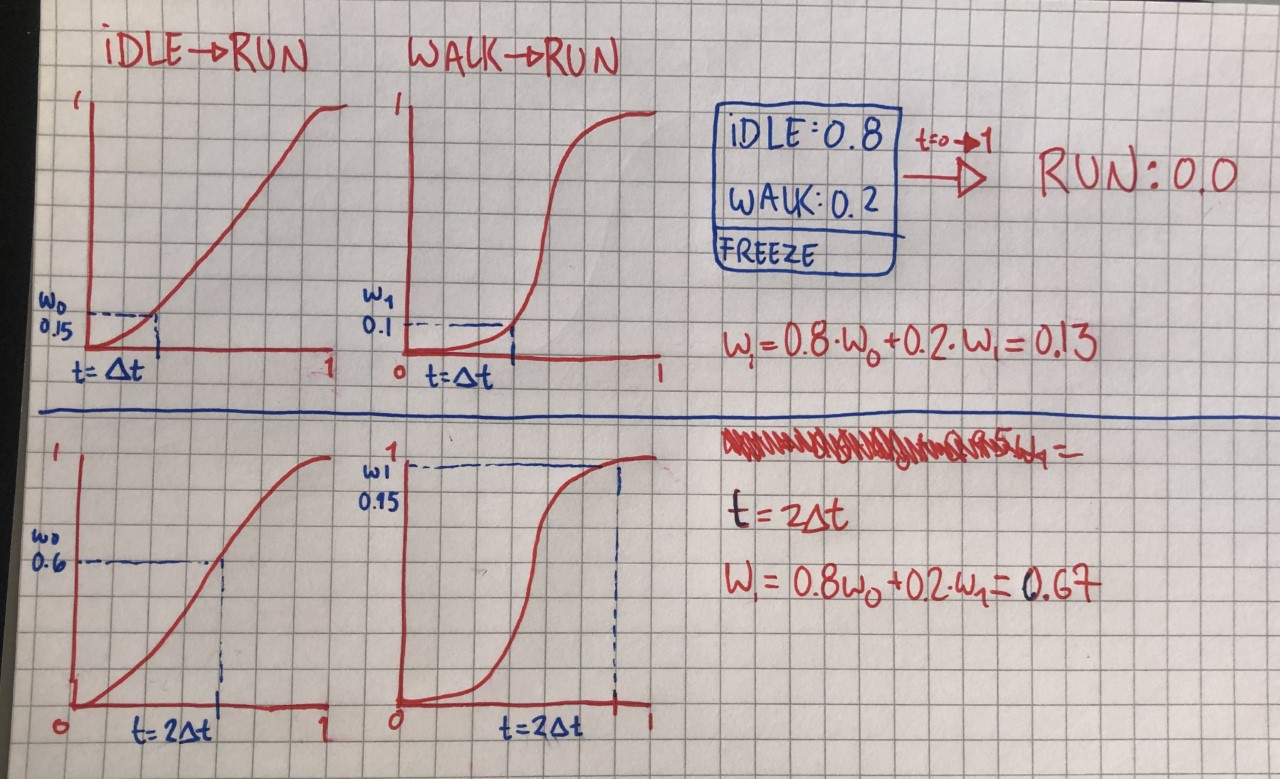
\includegraphics[width=\textwidth]{frozen-transitions}
  \caption{Frozen transition}
  \label{fig:frozen-transition}
\end{figure*}
To evaluate $step$ we notice that each $l\in\mathcal{L}$ should provide update routines $\dot{p}^*=l_{p,m}(\mathcal{A},\mathcal{C})$ and $\dot{r}^*=l_{r,m}(\mathcal{A},\mathcal{C})$ which are then combined.
\begin{equation}
\begin{split}
\dot{p}*&=\sum_{0<=k<m}\omega_k*l_{p,k}(\mathcal{A},\mathcal{C})\\
\dot{r}*&=\sum_{0<=k<m}\omega_k*l_{r,k}(\mathcal{A},\mathcal{C})\\
\end{split}
\end{equation}
The values can be inserted directly back into $\mathcal{A}$ while $p$ and $r$ are update with a forward Euler step using $\Delta{t}$. As before the update routines can be arbitrarily complex, which is natural given the idiosyncracity of human movement. As such our choise of expressiveness in these function are imposing limits on the types of locomotion we are able to model. We use a simple yet expressive apporach common to game development.   

velocity, velocity damper function, movement spring constant, orientation spring constant

velocity magnitude depends on the amount angular rotation. Slower when curving
move from current velocity to requested velocity is handled by spring.
move from orientation to requested orientation handled by soring.
Parameters are velocity, velocity damper function, velocity spring constant, orientation spring constant.


Notice that the formulation for $D$ is generic. In production a mapping between the generic movement model and a more context specific model would usually be needed. 

\subsection{missing}
Add animator constraint to model ? Example is 180. We dont start moving backwards immediately. First we rotate 90 degrees on the spot and then we start a 90 degree run to idle movement
Handle this by setting limits on rotation relative to forward movement ? Better to have a locomotion mode where velocity magnitude is 0 when facing relative to direction i < threshold.

Clear description of entire parameter set

Show very clear example. Pseudo code with idle and walk state. 